\section{Introduction}

Speech pronunciation assessment plays a crucial role in language learning~\cite{kheir-etal-2023-automatic, truong04_icall} and diagnosis of speech disorders~\cite{ssdm}. As traditional human assessment is time-consuming and lacks unified standards, recent advancement has shifted to Computer-Aided Pronunciation Training (CAPT)~\cite{lee2016language-capt}.
Parallel to the bloom of textual large language models~\cite{OpenAI_chatgpt}, recent speech research focuses on audio-language foundation models~\cite{ji2024wavchat, huang2024dynamic} that unify multiple tasks including pronunciation assessment. However, little evidence shows that multi-task learning improves performance in specific tasks like pronunciation modeling. Thus, \textit{automatic pronunciation assessment remains a task-specific area} requiring domain-specific priors in model design.

Automatic pronunciation assessment involves detecting multiple aspects of speech quality~\cite{lee2016language-capt}, including fluency, intonation, phonetic errors, prosodic features, stress patterns, and rhythmic consistency. We focus on a core module: phonetic error detection, which aims to identify pronunciation deviations at a fine-grained phoneme level. This is fundamentally an \textit{allophony} problem~\cite{boomershine2008impact-allophony}. Specifically, if a person pronounces phoneme A, how confidently can we determine its relation to phoneme $\hat{A}$? For instance, can AI models reliably distinguish between your pronunciation of the phoneme ``TH'' when the ground truth is ``S'' in the word \textit{think}, as illustrated in Figure~\ref{fig:demo}? So far, we have found no evidence of such capabilities in mainstream language learning platforms such as Duolingo~\cite{Duolingo}, Speak~\cite{SpeakApp}, or even GPT-4o Voice~\cite{OpenAI_GPT4o}. 

Earlier studies have treated pronunciation allophony as a phoneme recognition or classification task, using normalized classification logits scores as confidence measures~\cite{ssdm,yang22v_interspeech, lian2023unconstrained-udm, lian-anumanchipalli-2024-towards-hudm,lian2024ssdm2.0}. These are also called phonetic replacement errors in dysfluency modeling~\cite{lian2023unconstrained-udm, lian-anumanchipalli-2024-towards-hudm, zhou24eyolostutter, zhou2024stutter-solver, zhou2024timetokensbenchmarkingendtoend, ssdm, lian2024ssdm2.0,zhang2025analysisevaluationsyntheticdata, guo2025dysfluentwfstframeworkzeroshot, ye2025seamlessalignment-neurallcs, 11036667}. While~\cite{lee2025dypcl} explored phoneme similarity in CTC training for dysarthric speech, their approach focuses on transcribing what speakers should have said rather than what they actually said, which is our research focus. Another relevant work~\cite{choi2025leveragingallophonyselfsupervisedspeech} demonstrated that self-supervised speech representations can implicitly leverage phoneme similarity in a way that aligns more closely with human perception. However, it primarily focused on analysis and still fails to transcribe what the person actually said. Our work, on the other hand, focuses on the latter task, which is \textit{distinct} and more \textit{challenging}.

\begin{figure}[t]
    \centering
    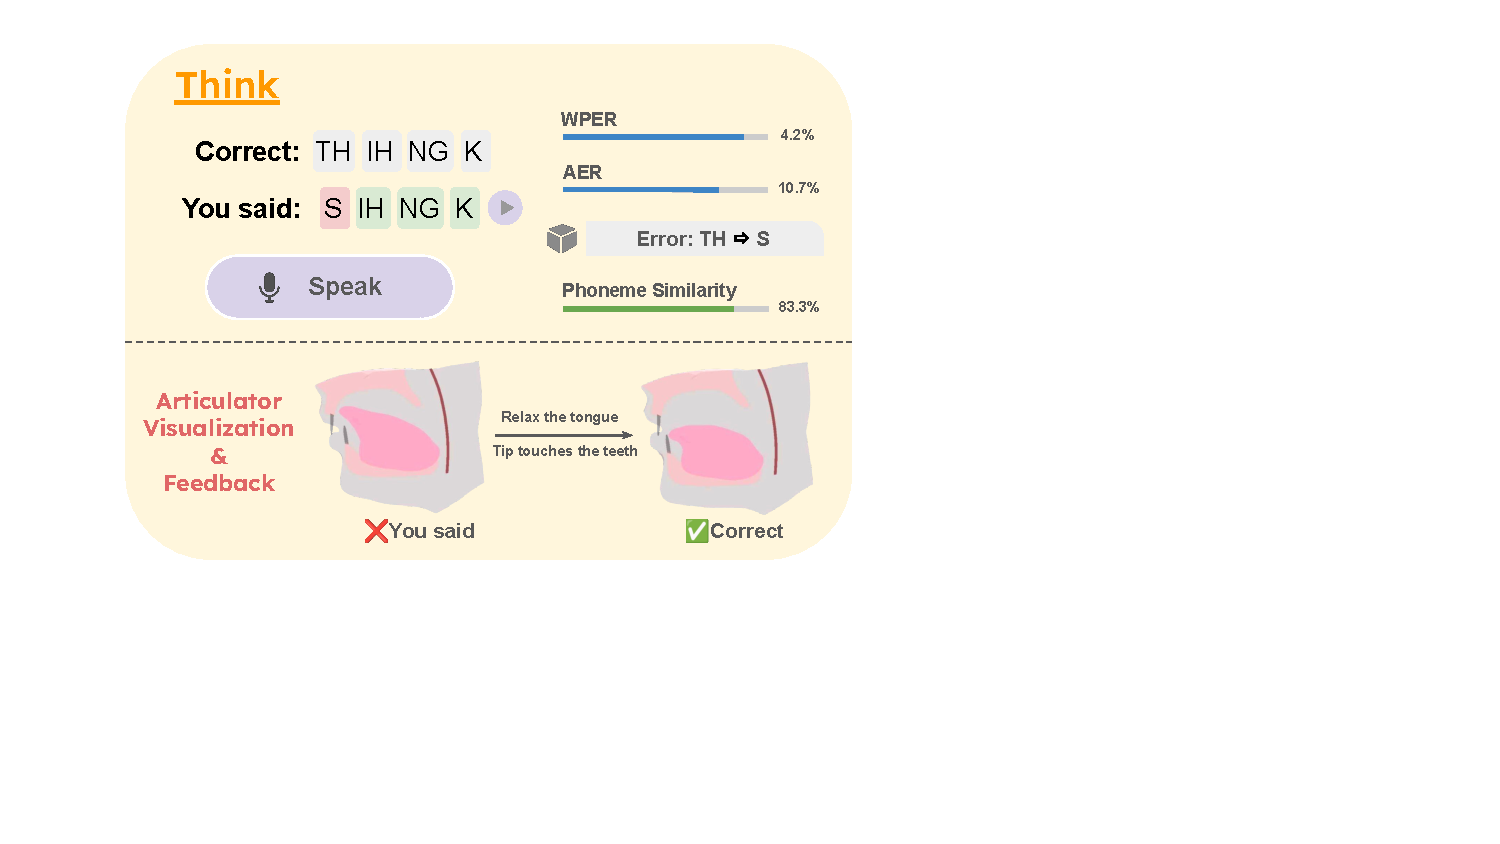
\includegraphics[height=4.8cm]{img/demo3.pdf}
    \vspace{-5pt}
    \caption{Demo of our method. Model transcribes user speech into phoneme sequences, detects errors, scores using metrics, and generates articulator visualizations and feedback~\cite{cho2024jstsp}: relax the tongue and place it against the roof of the mouth, with the tip lightly touching the teeth.}
    \label{fig:demo}
\end{figure}

In this paper, we propose a framework for verbatim phoneme recognition with phoneme similarity modeling, trained using multi-task learning~\cite{crawshaw2020multitasklearningdeepneural}: phoneme mapping and connectionist
temporal classification (CTC), aiming to accurately transcribe the phonemes pronounced by the speaker.
Phoneme similarity modeling, which serves as a method to reveal allophony information, better aligns with both how humans produce speech and how the human ear perceives it. We thus propose three novel phoneme similarity modeling methods: heuristic-based, articulatory-based, and Sylber-based~\cite{cho2024sylber} methods. Through this modeling, we compute the similarity score between each pair of phonemes. The process of integrating phoneme similarity into the training procedure is referred to as \textit{soft-training}.
To providing training material that incorporates phonetic errors and accurate labels, we follow the TTS-based simulation approach~\cite{zhou24eyolostutter} and generate a simulated dataset with vowel and consonant substitutions, which we named \textit{VCTK-accent} and open-sourced. In addition, We introduce two novel metrics: \textit{WPER} and \textit{AER}, which can be used not only for evaluating phoneme recognition models but also as pronunciation assessment scores for speech.

Evaluated on the VCTK-accent test sets and real speech datasets, our method shows impressive performance. Our training strategy-\textit{multi-task learning \& soft-training} significantly reduced the PER, WPER, and AER, proving its effectiveness. This highlights the crucial role of phoneme similarity modeling as a key approach to tackling the problem. Our work establishes a new benchmark for phonetic error detection. The project page is available
at \url{https://berkeley-speech-group.github.io/Phonetic-Error-Detection/}.